\chapter{Análisis exploratorio de datos complementario}

En este anexo se presentan resúmenes tabulados y gráficos de los datos utilizados y las elecciones consideradas con el objetivo de complementar, para el lector interesado, el análisis exploratorio de los datos. 

\section*{Resultados generales de las 4 elecciones}

En esta sección presento unas tablas de resumen de los resultados electorales oficiales del Ministerio del Interior francés para las 4 elecciones consideradas en el análisis. Podemos ver las votaciones tanto en las primeras como en las segundas vueltas y para todas las etiquetas políticas. 

\begin{table}[H]
\centering
\resizebox{\linewidth}{!}{
\begin{tabular}{l c r r r r}
\multicolumn{6}{c}{\textbf{Elecciones Presidenciales 2007}} \\[5pt] 
\multirow{2}{*}{\textbf{Candidato(a)}} & 
\multirow{2}{*}{\textbf{Partido}} & 
\multicolumn{1}{c}{\textbf{Votos}} & \textbf{\% Ef.} & 
\multicolumn{1}{c}{\textbf{Votos}} & \textbf{\% Ef.}\\ 
& &  
\multicolumn{2}{c}{1ra vuelta} & 
\multicolumn{2}{c}{2da vuelta} \\[2pt] 
\hline
 & & & & & \\[\dimexpr-\normalbaselineskip+3pt]
Nicolas Sarkozy & UMP & 11,448,663 & 31.18 & 18,983,138 & 53.06 \\
Ségolène Royal & PS & 9,500,112 & 25.87 & 16,790,440 & 46.94\\
\hdashline
François Bayrou & UDF & 6,820,119 & 18.57 & & \\
Jean Marie Le Pen & FN & 3,834,530 & 10.44 & & \\
Olivier Besancenot & LRO & 1,498,581 & 4.08 & & \\
Philippe de Villiers & MPF & 818,407 & 2.23 & & \\
Marie-George Buffet & PC & 707,268 & 1.93 & & \\
Dominique Voynet & Verts & 576,666 & 1.57 & & \\
Arlette Laguiller & LO & 487,857 & 1.33 & & \\
José Bové & Indep. & 483,008 & 1.32 & & \\
Frédérick Nihous & CPNT & 420,645 & 1.15 & & \\
Gérard Schivardi & PT & 123,540 & 0.34 & & \\[3pt]
\hline
 & & & & & \\[\dimexpr-\normalbaselineskip+3pt]
\multicolumn{2}{l}{\textbf{Votación efectiva}} 
& 36,719,396 &
& 35,773,578 & \\
\multicolumn{2}{l}{Blancos o nulos} 
& 534,846 & 
& 1,568,426 & \\[3pt]
\hline
 & & & & & \\[\dimexpr-\normalbaselineskip+3pt]
\multicolumn{2}{l}{\textbf{Votación emitida}} 
& 37,254,242 & 
& 37,342,004 & \\
\multicolumn{2}{l}{Abstenciones} 
& 7,218,592 & 
& 7,130,729 & \\[3pt]
\hline
 & & & & & \\[\dimexpr-\normalbaselineskip+3pt]
\multicolumn{2}{l}{\textbf{Lista nominal}} 
& 44,472,834 & 
& 44,472,733 & \\
\end{tabular}
}
\caption{Resultados de las elecciones presidenciales francesas de 2007, resultando presidente electo Nicolas Sarkozy (UMP). Fuente: elaboración propia con los datos oficiales del Ministerio del Interior.}
\label{tbl:Resul_Oficiales_P07}
\end{table}

\begin{sidewaystable}[ph!]
\centering
\resizebox{\linewidth}{!}{
\begin{tabular}{l c r r c r r c c}
\multicolumn{9}{c}{\textbf{Elecciones Legislativas 2007}} \\[5pt] 
\multicolumn{2}{c}{\multirow{2}{*}{\textbf{Plataforma política}}} & 
\textbf{Votos} & 
\textbf{\% Ef.} & 
\textbf{Asientos} &
\textbf{Votos} & 
\textbf{\% Ef.} & 
\textbf{Asientos} &
\multirow{2}{*}{\textbf{Total de Asientos}}\\ 
\multicolumn{2}{c}{} 
& \multicolumn{3}{c}{1ra vuelta} 
& \multicolumn{3}{c}{2da vuelta} 
& \\[2pt] 
\hline
 & & & & & & & &\\[\dimexpr-\normalbaselineskip+3pt]
Union pour un Mouvement Populaire & UMP 
& 10,289,737 & 39.54 & 98 & 9,460,710 & 46.36 & 215 & 313 \\
Socialiste & SOC 
& 6,436,520 & 24.73 & 1 & 8,624,861 & 42.27 & 185 & 186 \\
Majorité Présidentielle & MAJ
& 616,440 & 2.37 & 8 & 433,057 & 2.12 & 14 & 22\\
Parti Communiste Français & COM 
& 1,115,663 & 4.29 & - & 464,739 & 2.28 & 15 & 15\\
Divers Gauche & DVG
& 513,407 & 1.97 & - & 503,556 & 2.47 & 15 & 15\\
Divers Droite & DVD 
& 641,842 & 2.47 & 2 & 238,588 & 1.17 & 7 & 9\\
Radicales de Gauche & RDG
& 343,565 & 1.32 & - & 333,194 & 1.63 & 7 & 7\\
Les Verts & VEC
& 845,977 & 3.25 & - & 90,975 & 0.45 & 4 & 4\\
Union pour la Démocratie Française & UDFD 
& 1,981,107 & 7.61 & - & 100,115 & 0.49 & 3 & 3\\
Mouvement pour la France & MPF
& 312,581 & 1.20 & 1 & - & - & - & 1\\
Divers & DIV 
& 267,760 & 1.03 & - & 33,068 & 0.16 & 1 & 1\\
Régionaliste & REG
& 133,473 & 0.51 & - & 106,484 & 0.52 & 1 & 1\\
Front National & FN 
& 1,116,136 & 4.29 & - & 17,107 & 0.08 & - & -\\
Extrême Gauche & EXG 
& 888,250 & 3.41 & - & -  & - & - & -\\
Chase Pêche Nature Traditions & CPNT 
& 213,427 & 0.82 & - & - & - & - & -\\
Ecologistes & ECO 
& 208,456 & 0.80 & - & - & - & - & -\\
Extrême Droite & EXD 
& 102,124 & 0.39 & - & - & - & - & -\\[3pt]
\hline
 & & & & & & & & \\[\dimexpr-\normalbaselineskip+3pt]
\multicolumn{2}{l}{\textbf{Votación efectiva}} 
& 26,026,465 & &
& 20,406,454 & & & \\
\multicolumn{2}{l}{Blancos o nulos} 
& 495,357 & &
& 722,585 & & & \\[3pt]
\hline
 & & & & & & & &\\[\dimexpr-\normalbaselineskip+3pt]
\multicolumn{2}{l}{\textbf{Votación emitida}} 
& 26,521,822 & &
& 21,129,039 & & & \\
\multicolumn{2}{l}{Abstenciones} 
& 17,374,011 & &
& 14,096,209 & & & \\[3pt]
\hline
 & & & & & & &\\[\dimexpr-\normalbaselineskip+3pt]
\multicolumn{2}{l}{\textbf{Lista nominal}} 
& 43,895,833 & &
& 35,225,248 & & & \\
\end{tabular}
}
\caption{Resultados de las elecciones legislativas de 2007 para el conjunto de todo el territorio francés, incluyendo el ultramar. Fuente: elaboración propia con los datos oficiales del Ministerio del Interior.}
\label{tbl:Resul_Oficiales_L07}
\end{sidewaystable}

\begin{table}[H]
\centering
\resizebox{\linewidth}{!}{
\begin{tabular}{l c r r r r}
\multicolumn{6}{c}{\textbf{Elecciones Presidenciales 2012}} \\[5pt] 
\multirow{2}{*}{\textbf{Candidato(a)}} & 
\multirow{2}{*}{\textbf{Partido}} & 
\multicolumn{1}{c}{\textbf{Votos}} & \textbf{\% Ef.} & 
\multicolumn{1}{c}{\textbf{Votos}} & \textbf{\% Ef.}\\ 
& &  
\multicolumn{2}{c}{1ra vuelta} & 
\multicolumn{2}{c}{2da vuelta} \\[2pt] 
\hline
 & & & & & \\[\dimexpr-\normalbaselineskip+3pt]
François Hollande & PS & 10,272,705 & 28.63 & 18,000,668 & 51.64\\
Nicolas Sarkozy & UMP & 9,753,629 & 27.18 & 16,860,685 & 48.36 \\
\hdashline
Marine Le Pen & FN & 6,421,426 & 17.90 & & \\
Jean-Luc Mélenchon & FG & 3,984,822 & 11.10 & & \\
François Bayrou & MoDem & 3,275,122 & 9.13 & & \\
Eva Joly & EELV & 828,345 & 2.31 & & \\
Nicolas Dupont-Aignan & DLR & 643,907 & 1.79 & & \\
Philippe Poutou & NPA & 411,160 & 1.15 & & \\
Nathalie Arthaud & LO & 202,548 & 0.56 & & \\
Jacques Cheminade & SP & 89,545 & 0.25 & & \\[3pt]
\hline
 & & & & & \\[\dimexpr-\normalbaselineskip+3pt]
\multicolumn{2}{l}{\textbf{Votación efectiva}} 
& 35,883,209 &
& 34,861,353 & \\
\multicolumn{2}{l}{Blancos o nulos} 
& 701,190 & 
& 2,154,956 & \\[3pt]
\hline
 & & & & & \\[\dimexpr-\normalbaselineskip+3pt]
\multicolumn{2}{l}{\textbf{Votación emitida}} 
& 36,584,399 & 
& 37,016,309 & \\
\multicolumn{2}{l}{Abstenciones} 
& 9,444,143 & 
& 9,049,998 & \\[3pt]
\hline
 & & & & & \\[\dimexpr-\normalbaselineskip+3pt]
\multicolumn{2}{l}{\textbf{Lista nominal}} 
& 46,028,542 & 
& 46,066,307 & \\
\end{tabular}
}
\caption{Resultados de las elecciones presidenciales francesas de 2012, resultando presidente electo François Hollande (PS). Fuente: elaboración propia con los datos oficiales del Ministerio del Interior.}
\label{tbl:Resul_Oficiales_P12}
\end{table}

\begin{sidewaystable}[ph!]
\centering
\resizebox{\linewidth}{!}{
\begin{tabular}{l c r r c r r c c}
\multicolumn{9}{c}{\textbf{Elecciones Legislativas 2012}} \\[5pt] 
\multicolumn{2}{c}{\multirow{2}{*}{\textbf{Plataforma política}}} & 
\textbf{Votos} & 
\textbf{\% Ef.} & 
\textbf{Asientos} &
\textbf{Votos} & 
\textbf{\% Ef.} & 
\textbf{Asientos} &
\multirow{2}{*}{\textbf{Total de Asientos}}\\ 
\multicolumn{2}{c}{} 
& \multicolumn{3}{c}{1ra vuelta} 
& \multicolumn{3}{c}{2da vuelta} 
& \\[2pt] 
\hline
 & & & & & & & &\\[\dimexpr-\normalbaselineskip+3pt]
Socialiste & SOC 
& 7,618,326 & 29.35 & 22 & 9,420,889 & 40.91 & 258 & 280 \\
Union pour un Mouvement Populaire & UMP 
& 7,037,268 & 27.12 & 9 & 8,740,628 & 37.95 & 185 & 194 \\
Divers Gauche & DVG
& 881,555 & 3.40 & 1 & 709,395 & 3.08 & 21 & 22\\
Europe-Écologie-Les Verts & VEC
& 1,418,264 & 5.46 & 1 & 829,036 & 3.60 & 16 & 17\\
Divers Droite & DVD 
& 910,034 & 3.51 & 1 & 417,940 & 1.81 & 14 & 15\\
Nouveau Centre & NCE
& 569,897 & 2.20 & 1 & 568,319 & 2.47 & 11 & 12\\
Radicales de Gauche & RDG
& 428,898 & 1.65 & 1 & 538,331 & 2.34 & 11 & 12\\
Front de Gauche & FG 
& 1,793,192 & 6.91 & - & 249,498 & 1.08 & 10 & 10\\
Parti Radical & PRV
& 321,124 & 1.24 & - & 311,199 & 1.35 & 6 & 6\\
Front National & FN 
& 3,528,663 & 13.60 & - & 842,695 & 3.66 & 2 & 2\\
Le Centre pour la France & CEN
& 458,098 & 1.77 & 1 & 113,196 & 0.49 & 2 & 2\\
Alliance Centriste & ALLI 
& 156,026 & 0.60 & - & 123,132 & 0.53 & 2 & 2\\
Régionaliste & REG
& 145,809 & 0.56 & - & 135,312 & 0.59 & 2 & 2\\
Extrême Droite & EXD 
& 49,499 & 0.19 & - & 29,738 & 0.13 & 1 & 1\\
Extrême Gauche & EXG 
& 253,386 & 0.98 & - & - & - & - & -\\
Ecologistes & ECO 
& 249,068 & 0.96 & - & - & - & - & -\\
Autres & AUT 
& 133,752 & 0.52 & - & - & - & - & -\\[3pt]
\hline
 & & & & & & & & \\[\dimexpr-\normalbaselineskip+3pt]
\multicolumn{2}{l}{\textbf{Votación efectiva}} 
& 25,952,859 & &
& 23,029,308 & & & \\
\multicolumn{2}{l}{Blancos o nulos} 
& 416,267 & &
& 923,178 & & & \\[3pt]
\hline
 & & & & & & & &\\[\dimexpr-\normalbaselineskip+3pt]
\multicolumn{2}{l}{\textbf{Votación emitida}} 
& 26,369,126 & &
& 23,952,486 & & & \\
\multicolumn{2}{l}{Abstenciones} 
& 19,712,978 & &
& 19,281,162 & & & \\[3pt]
\hline
 & & & & & & &\\[\dimexpr-\normalbaselineskip+3pt]
\multicolumn{2}{l}{\textbf{Lista nominal}} 
& 46,082,104 & &
& 43,233,648 & & & \\
\end{tabular}
}
\caption{Resultados de las elecciones legislativas de 2012 para el conjunto de todo el territorio francés, incluyendo el ultramar. Fuente: elaboración propia con los datos oficiales del Ministerio del Interior.}
\label{tbl:Resul_Oficiales_L12}
\end{sidewaystable}

\section*{Distribuciones del voto FN}

Adicionalmente a las distribuciones presentadas en el texto principal de la tesis, presento las distribuciones regionales y departamentale del voto frontista en el resto de las elecciones: 

\begin{figure}[h]
	\centering
	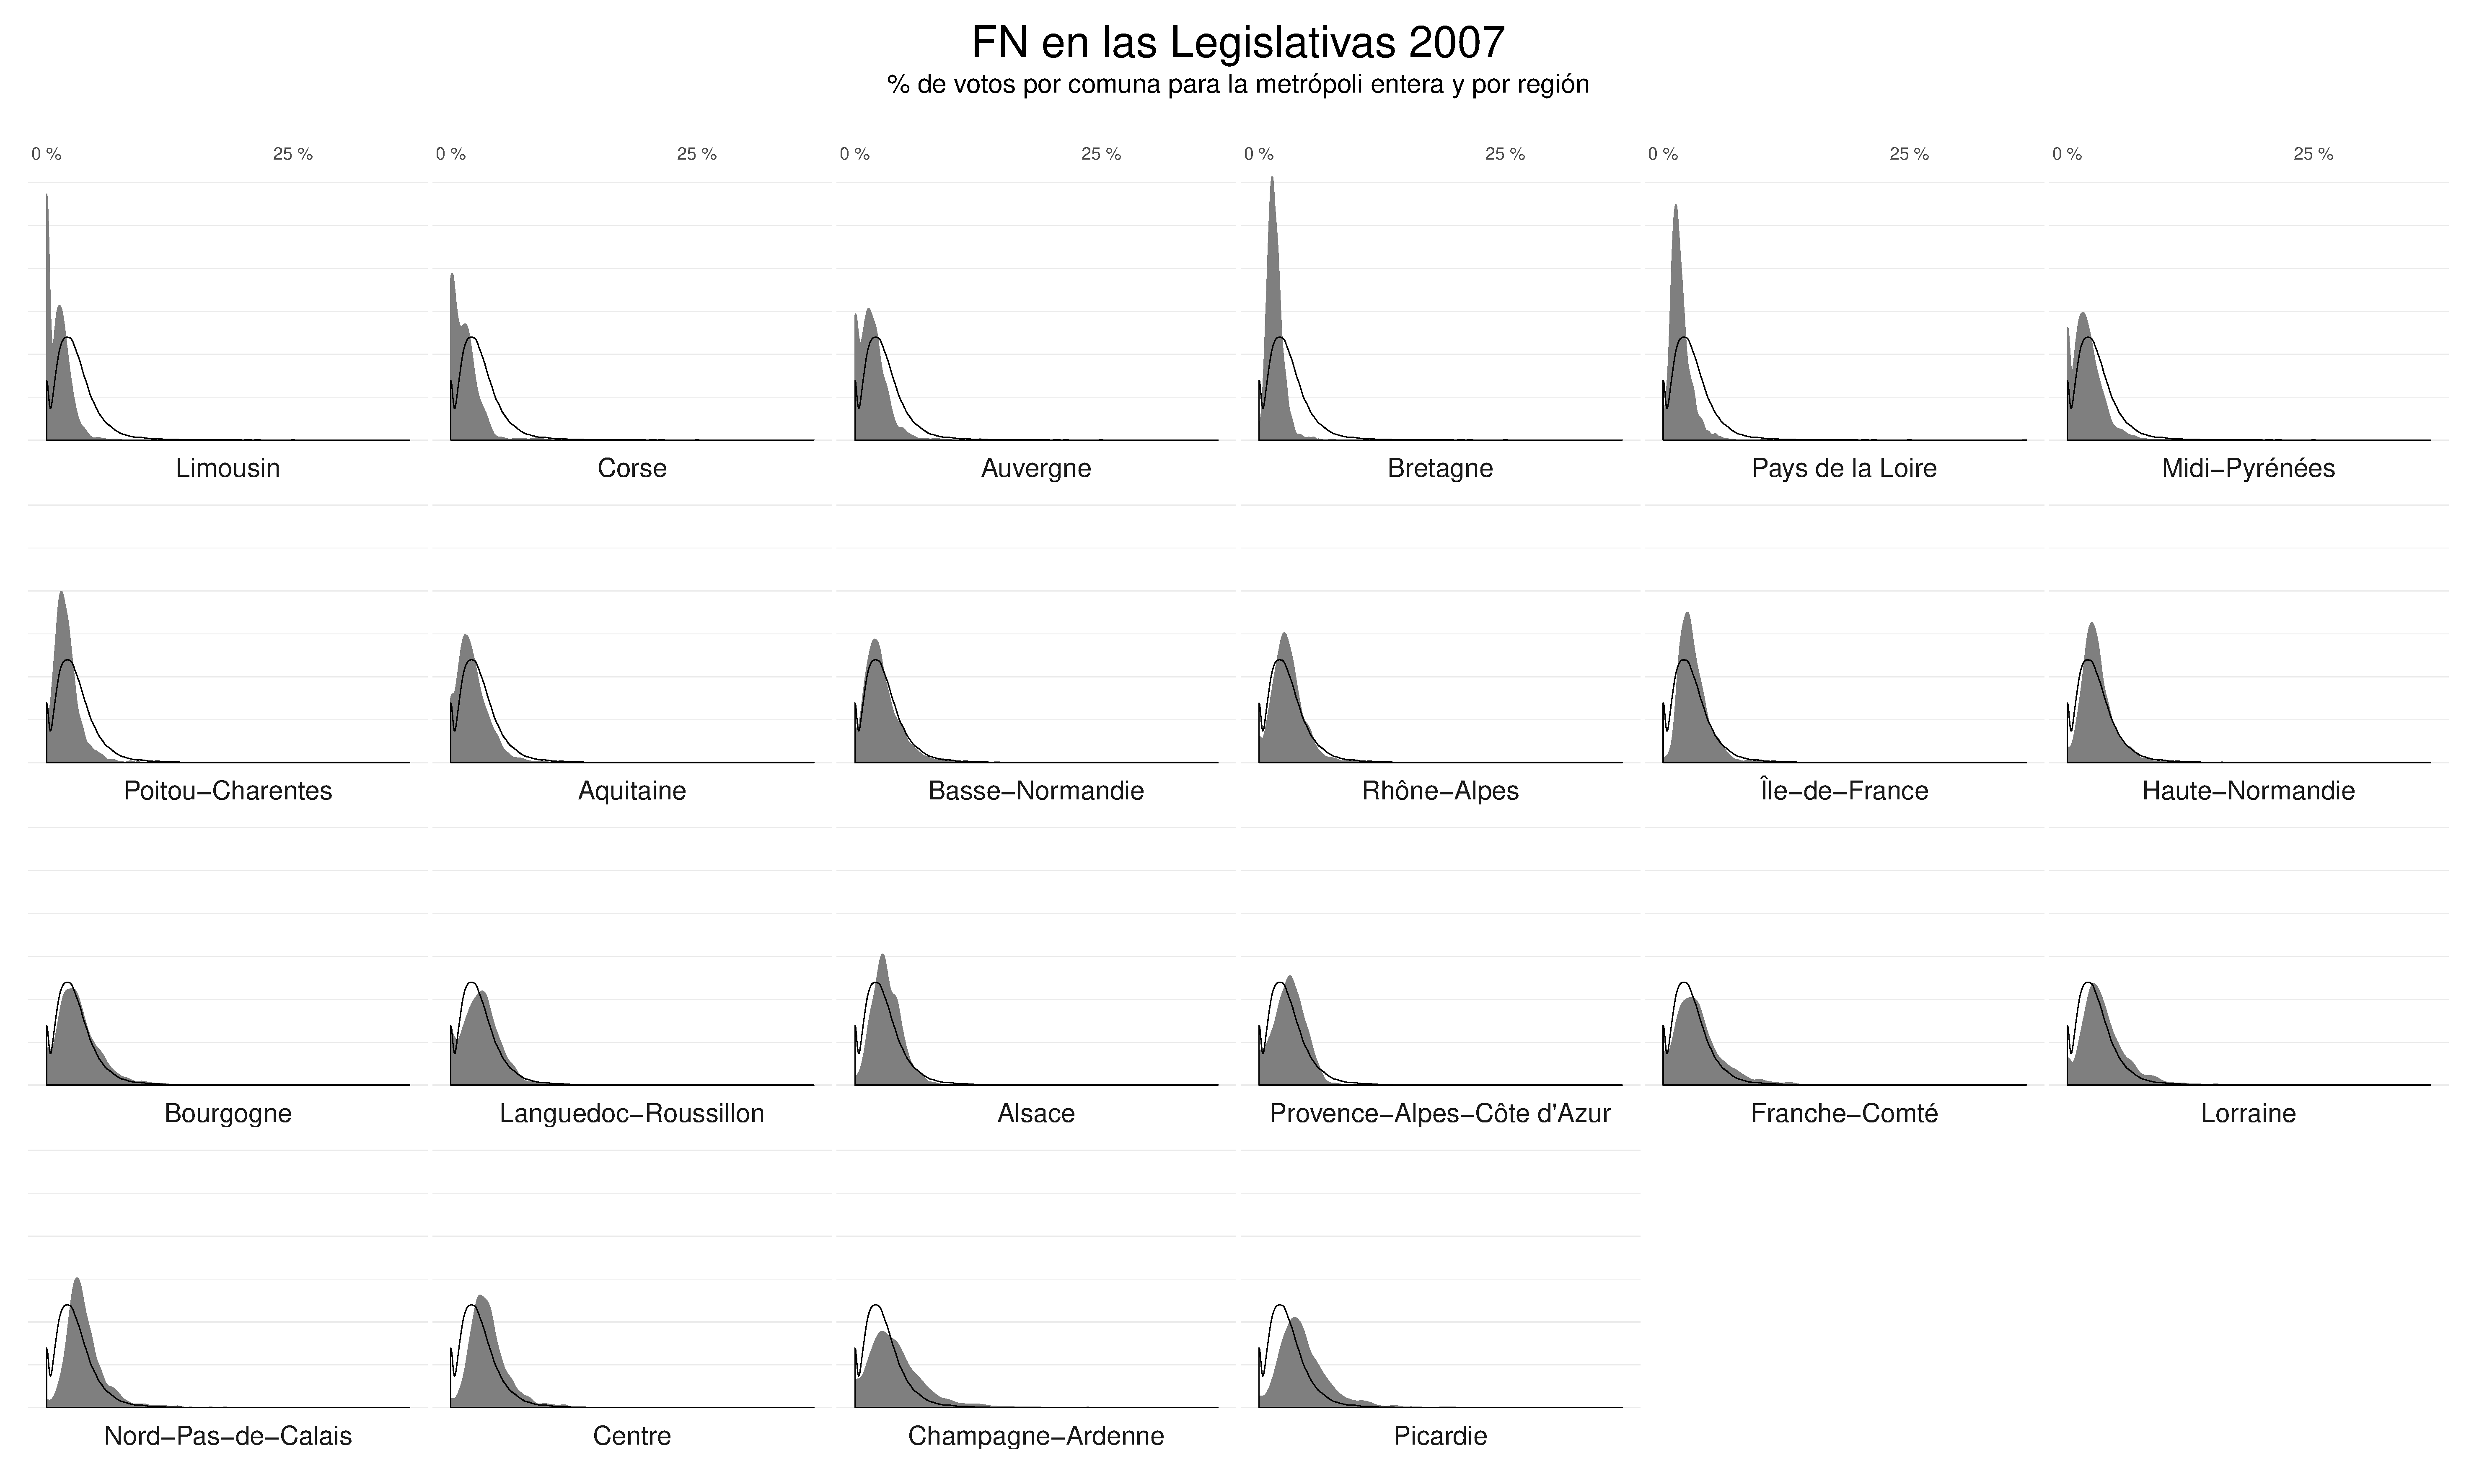
\includegraphics[scale=0.1]{Pct_Votos_Por_Comuna_FN_Reg_L07}
	\caption{Distribuciones regionales del porcentaje de votos recibidos por las candidaturas frontistas en las elecciones legislativas del 2007; las distribuciones rellenas de color son las distribuciones considerando solo las comunas de la región respectiva mientras que la distribución sin relleno es la distribución considerando todas las comunas de la metrópoli. Fuente: elaboración propia con base en los datos electorales oficiales del Ministerio del Interior francés.}
	\label{fig:Ej_Votos_Por_Reg_L07}	
\end{figure}

\begin{figure}[h]
	\centering
	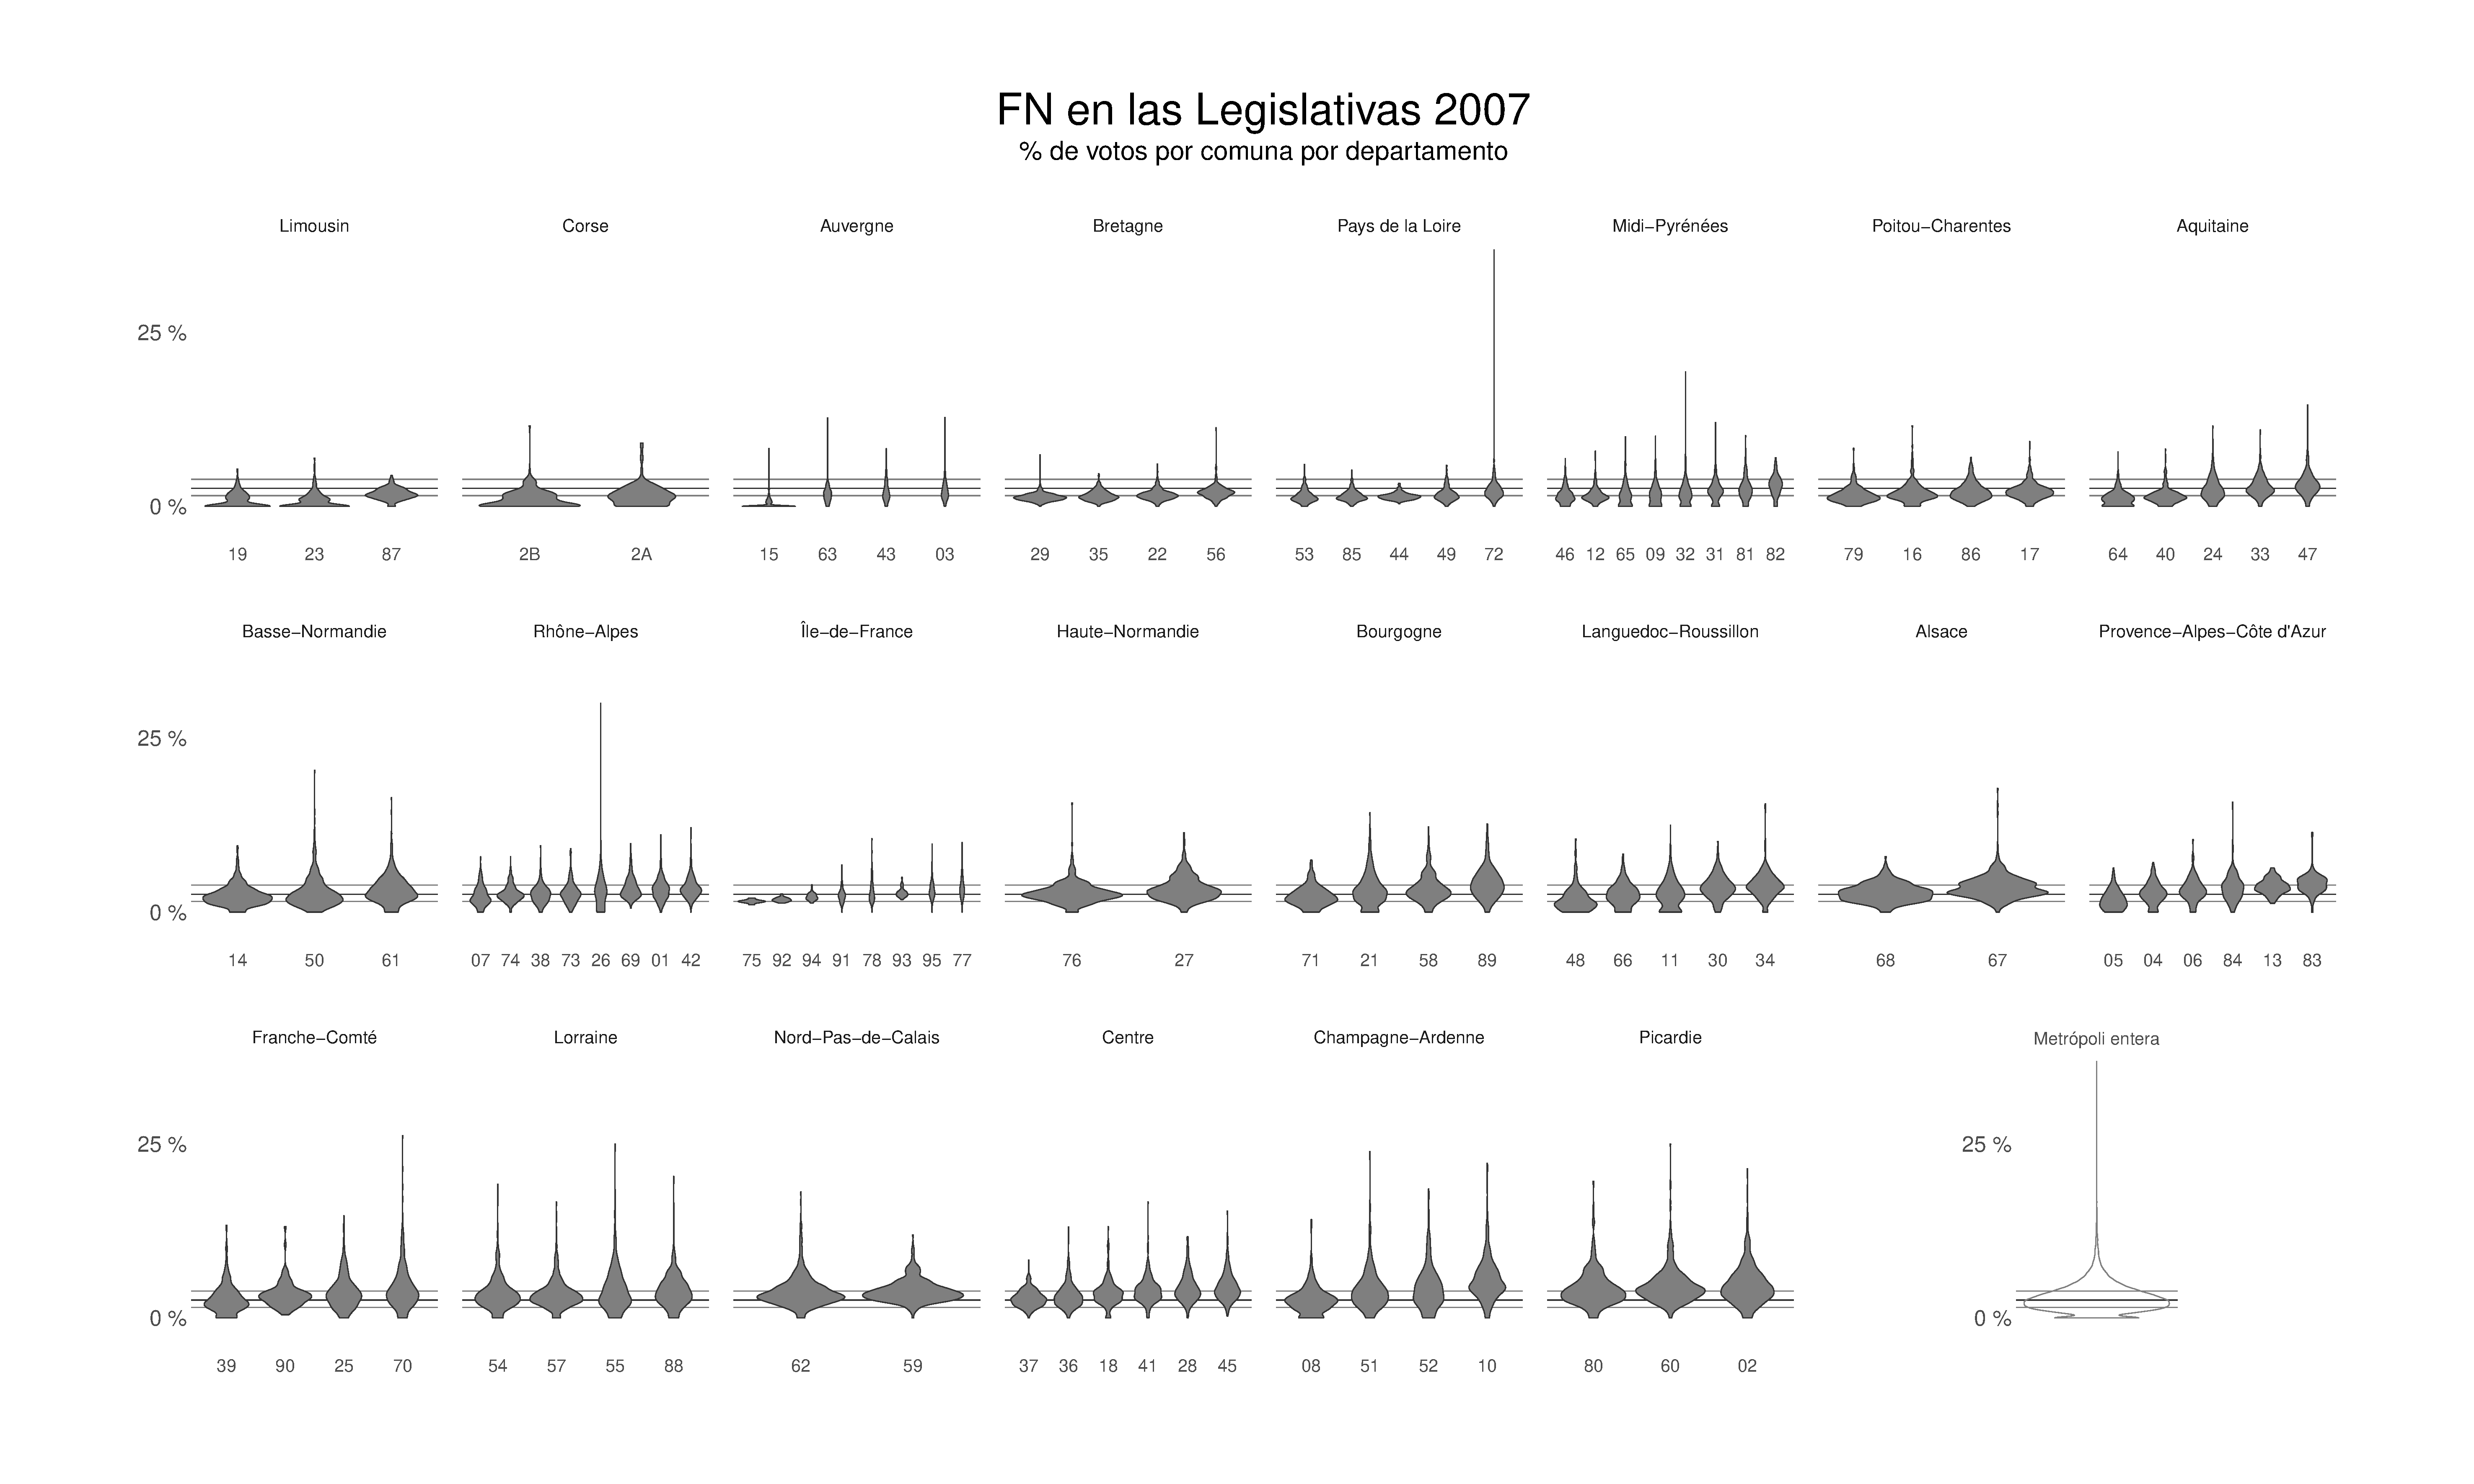
\includegraphics[scale=0.12]{Pct_Votos_Por_Comuna_FN_Dpto_L07}
	\caption{Distribuciones departamentales del porcentaje de votos recibidos por las candidaturas frontistas en las elecciones legislativas del 2007; los violines rellenos de color son las distribuciones considerando solo las comunas del departamento correspondiente mientras que las 3 líneas horizontales representan una referencia al rango intercuartílico y la mediana de la distribución considerando todas las comunas de la metrópoli, misma que puede verse en el panel inferior derecho. Fuente: elaboración propia con base en los datos electorales oficiales del Ministerio del Interior francés.}
	\label{fig:Ej_Votos_Por_Dpto_L07}	
\end{figure}

\begin{figure}[h]
	\centering
	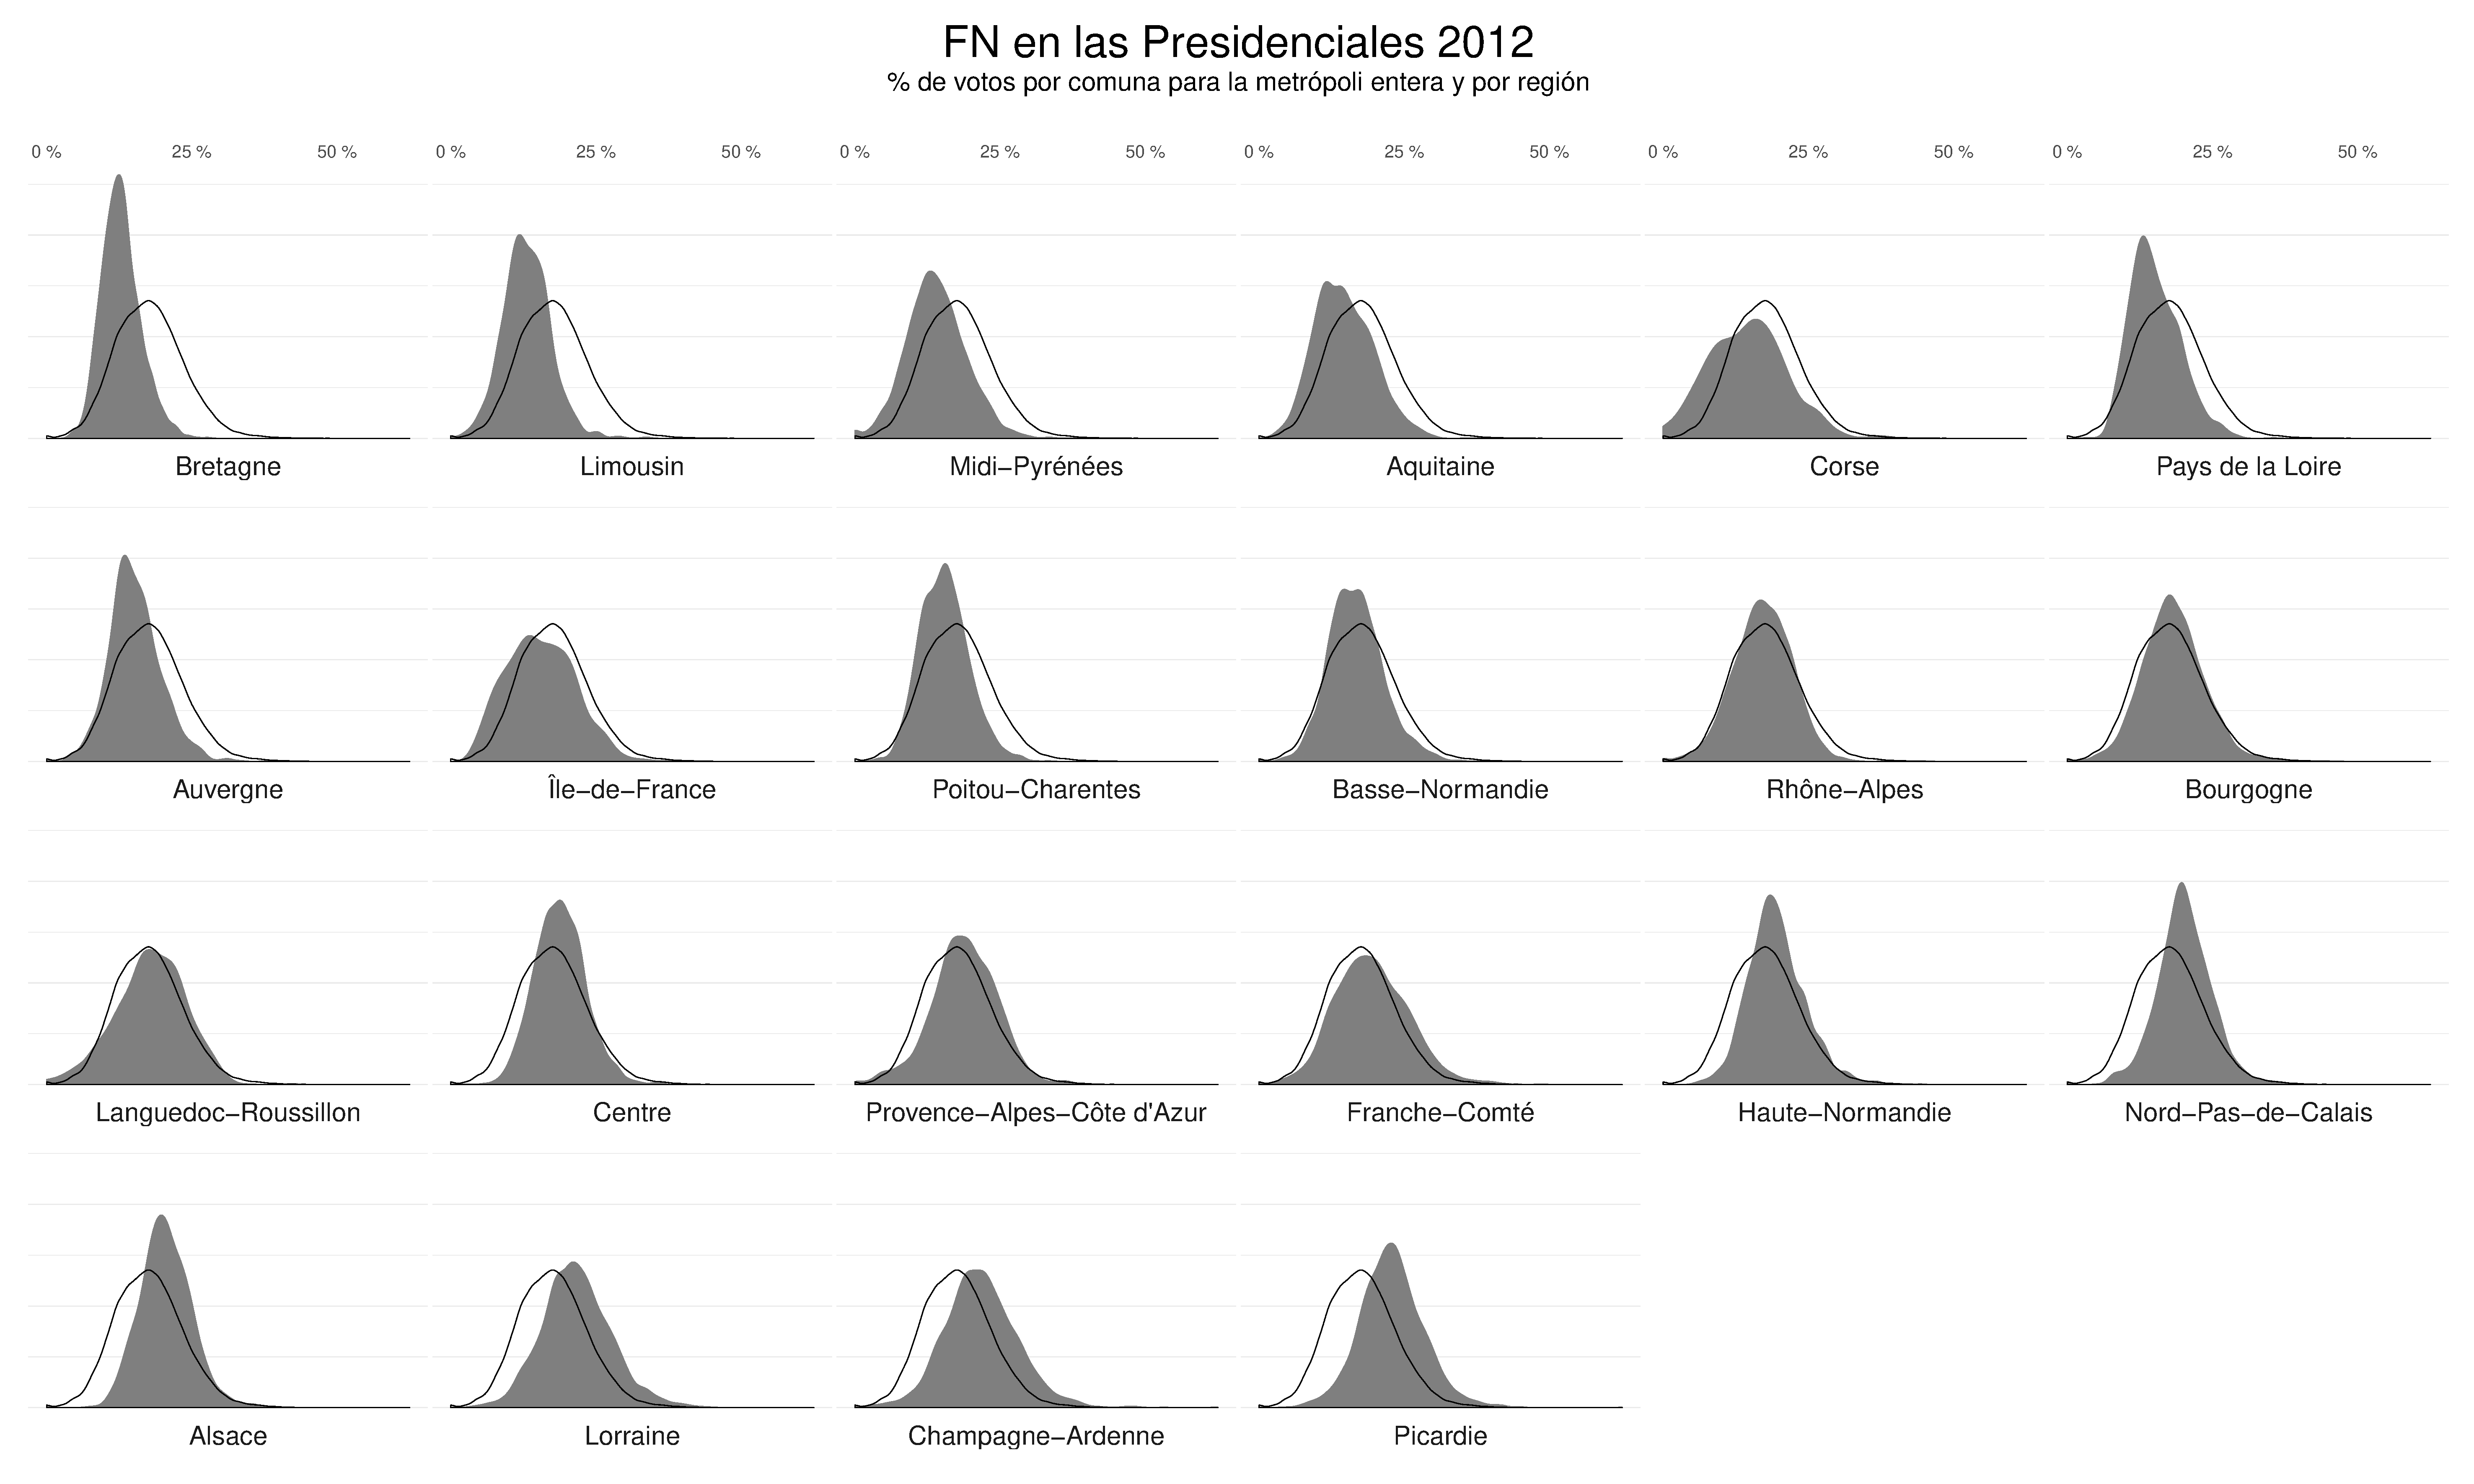
\includegraphics[scale=0.1]{Pct_Votos_Por_Comuna_FN_Reg_P12}
	\caption{Distribuciones regionales del porcentaje de votos recibidos por Marine Le Pen en las elecciones presidenciales del 2012; las distribuciones rellenas de color son las distribuciones considerando solo las comunas de la región respectiva mientras que la distribución sin relleno es la distribución considerando todas las comunas de la metrópoli. Fuente: elaboración propia con base en los datos electorales oficiales del Ministerio del Interior francés.}
	\label{fig:Ej_Votos_Por_Reg_P12}	
\end{figure}

\begin{figure}[h]
	\centering
	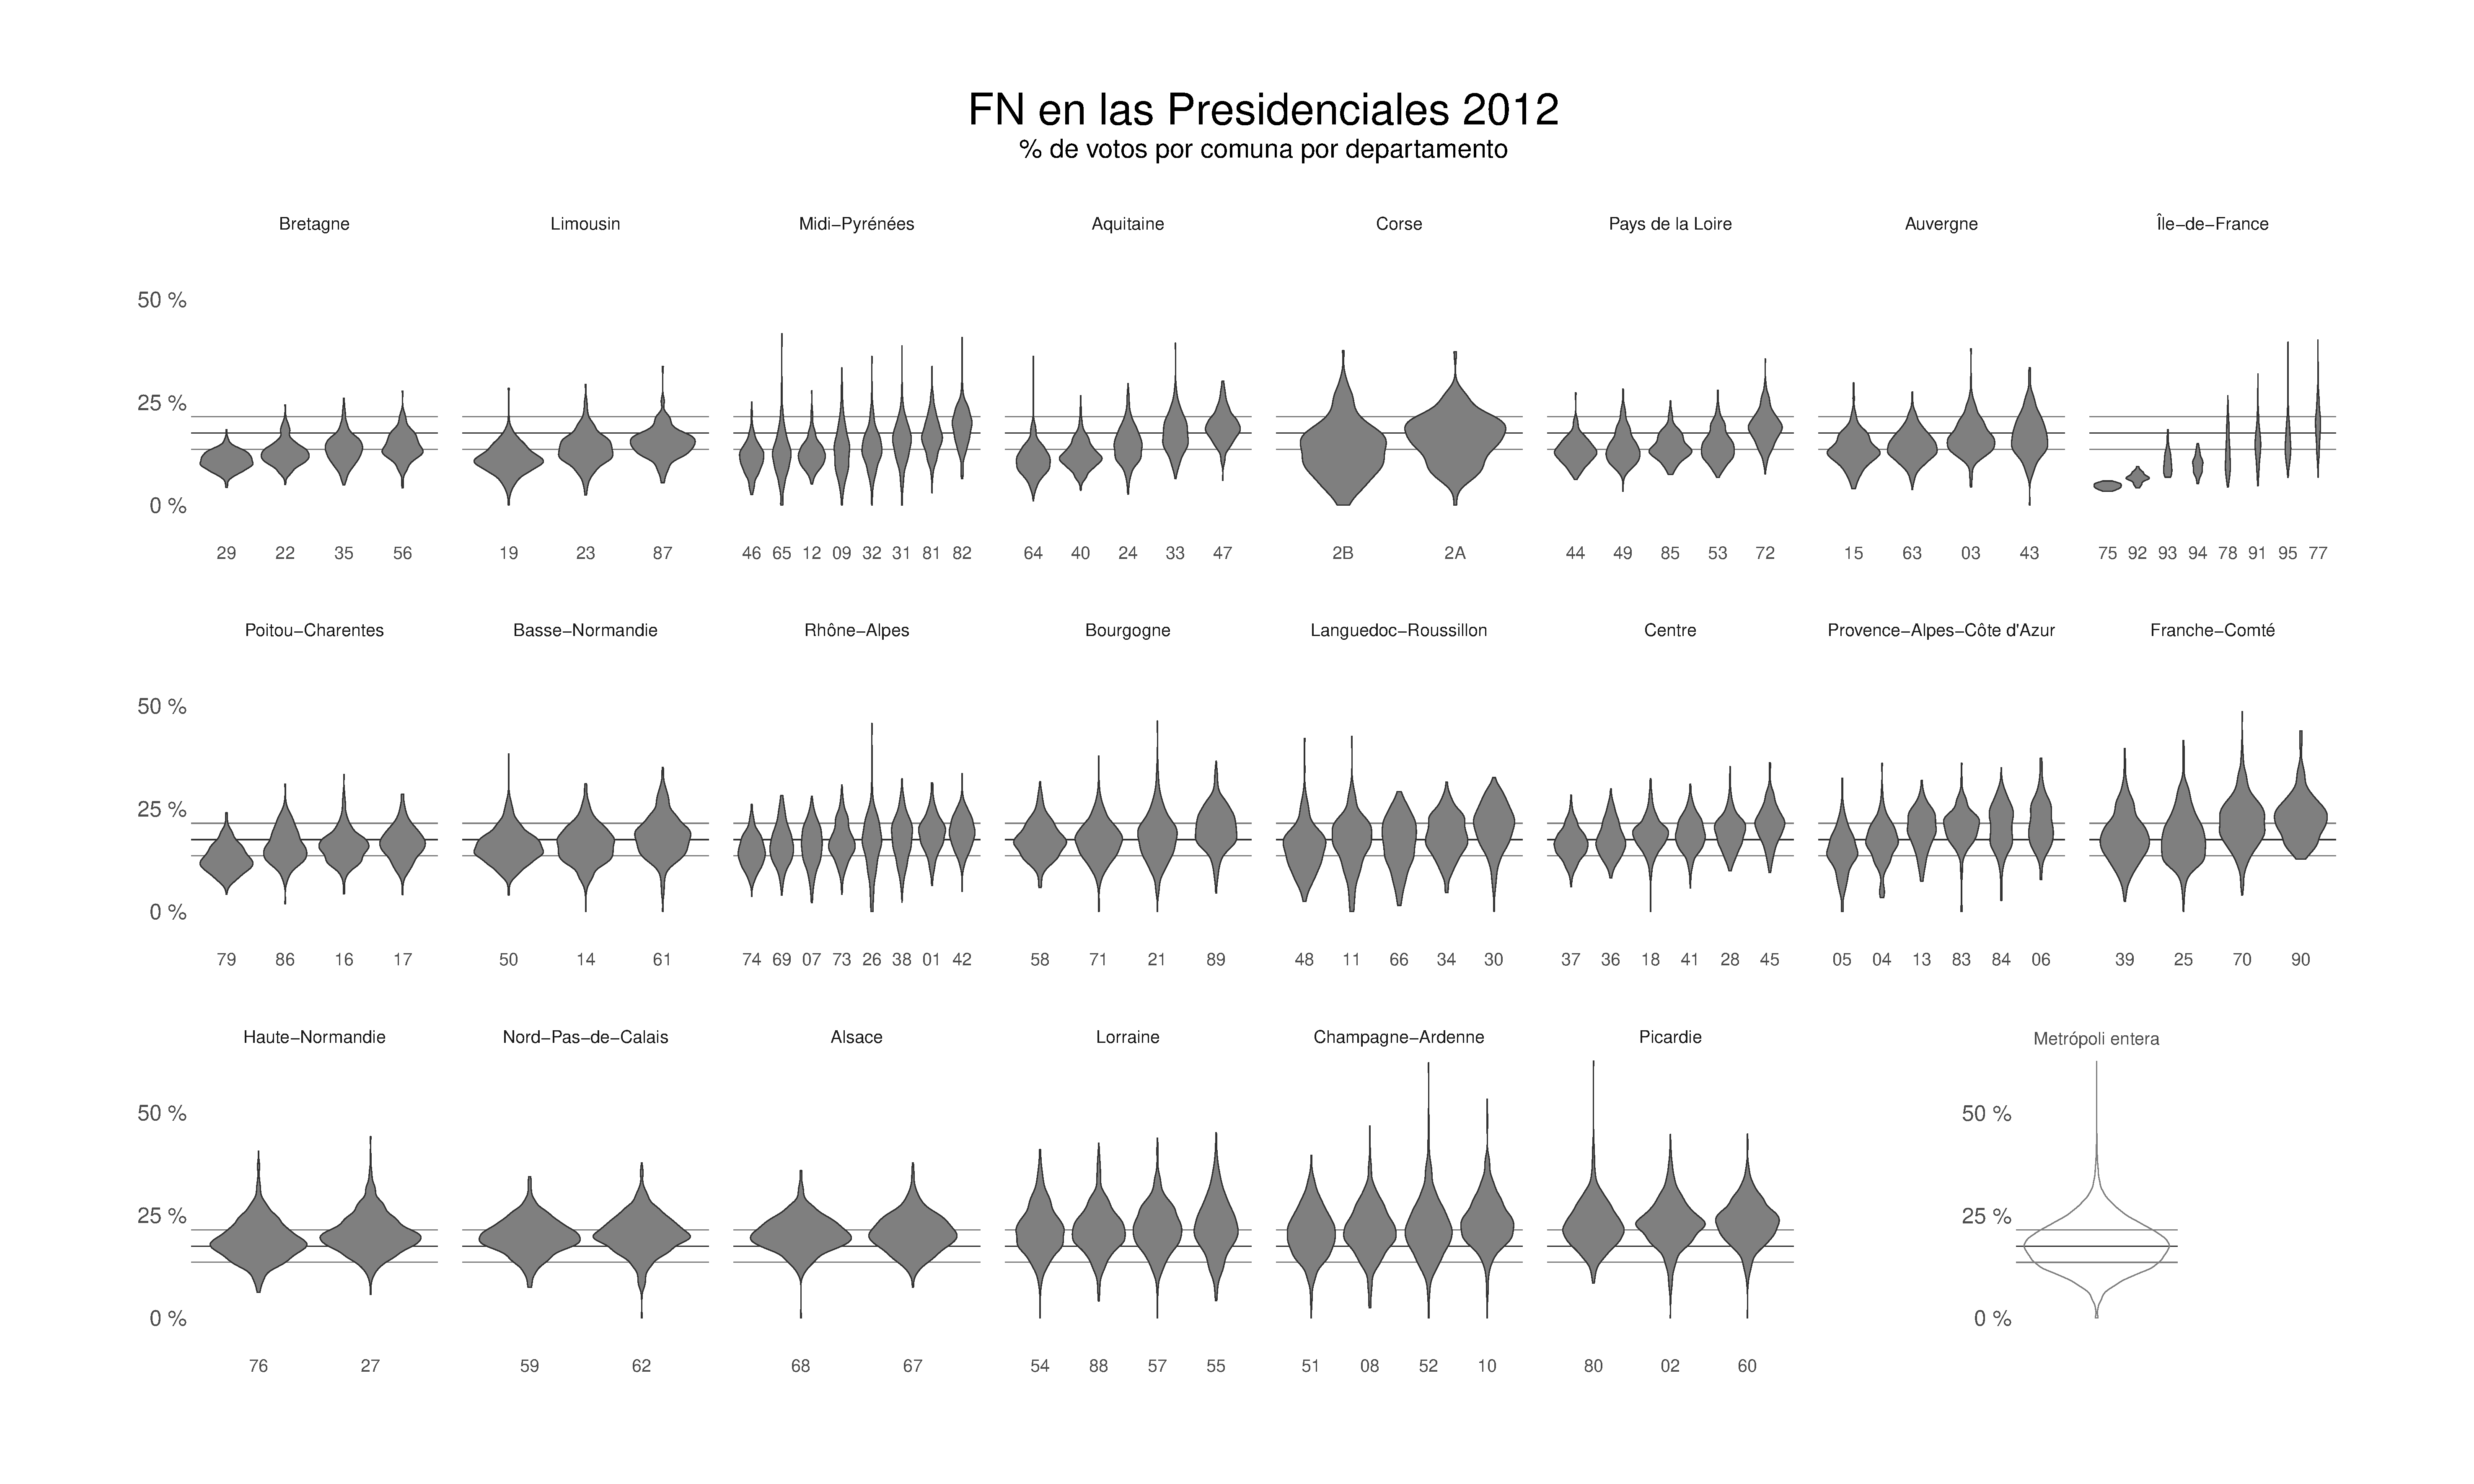
\includegraphics[scale=0.12]{Pct_Votos_Por_Comuna_FN_Dpto_P12}
	\caption{Distribuciones departamentales del porcentaje de votos recibidos por Marine Le Pen en las elecciones presidenciales de 2012; los violines rellenos de color son las distribuciones considerando solo las comunas del departamento correspondiente mientras que las 3 líneas horizontales representan una referencia al rango intercuartílico y la mediana de la distribución considerando todas las comunas de la metrópoli, misma que puede verse en el panel inferior derecho. Fuente: elaboración propia con base en los datos electorales oficiales del Ministerio del Interior francés.}
	\label{fig:Ej_Votos_Por_Dpto_P12}	
\end{figure}

\begin{figure}[h]
	\centering
	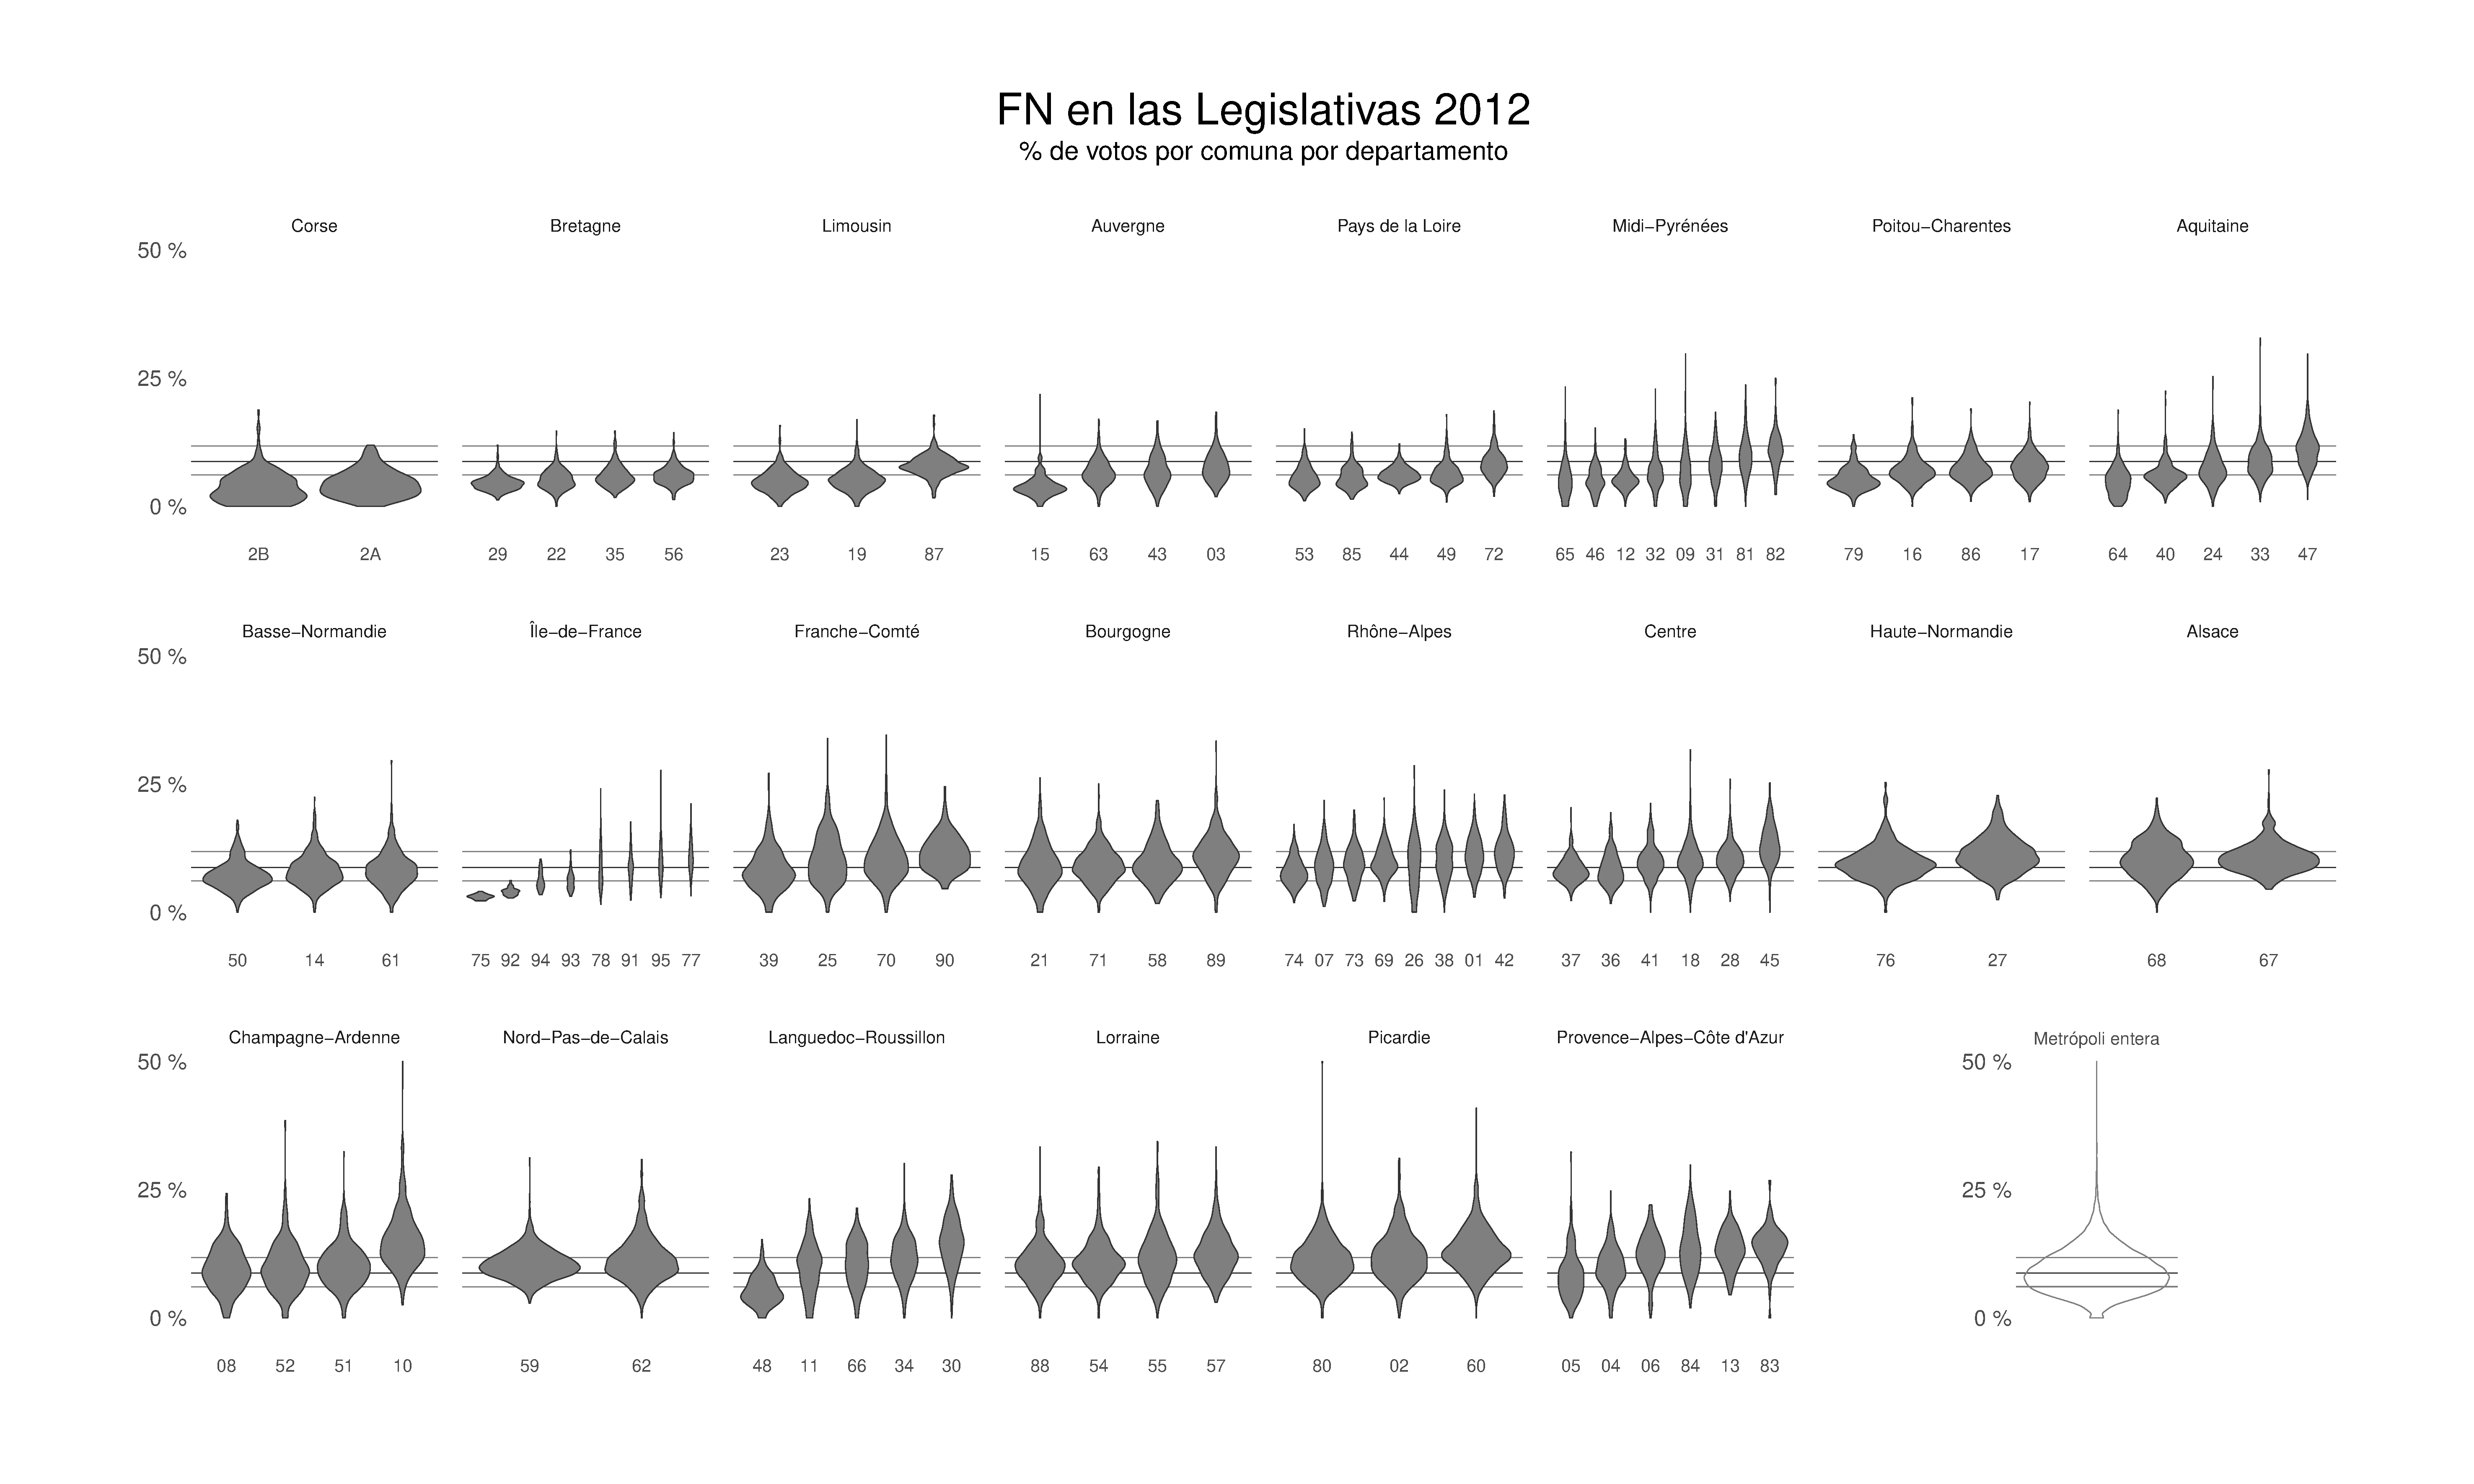
\includegraphics[scale=0.12]{Pct_Votos_Por_Comuna_FN_Dpto_L12}
	\caption{Distribuciones departamentales del porcentaje de votos recibidos por las candidaturas frontistas en las elecciones legislativas del 2012; los violines rellenos de color son las distribuciones considerando solo las comunas del departamento correspondiente mientras que las 3 líneas horizontales representan una referencia al rango intercuartílico y la mediana de la distribución considerando todas las comunas de la metrópoli, misma que puede verse en el panel inferior derecho. Fuente: elaboración propia con base en los datos electorales oficiales del Ministerio del Interior francés.}
	\label{fig:Ej_Votos_Por_Dpto_L12}	
\end{figure}